\subchapter{Installing the Codesourcery Lite toolchain}

\section{Getting the Toolchain}

Open a Browser and go to the \href{http://www.mentor.com/}{Mentor Graphics Homepage} \\
\begin{center}
  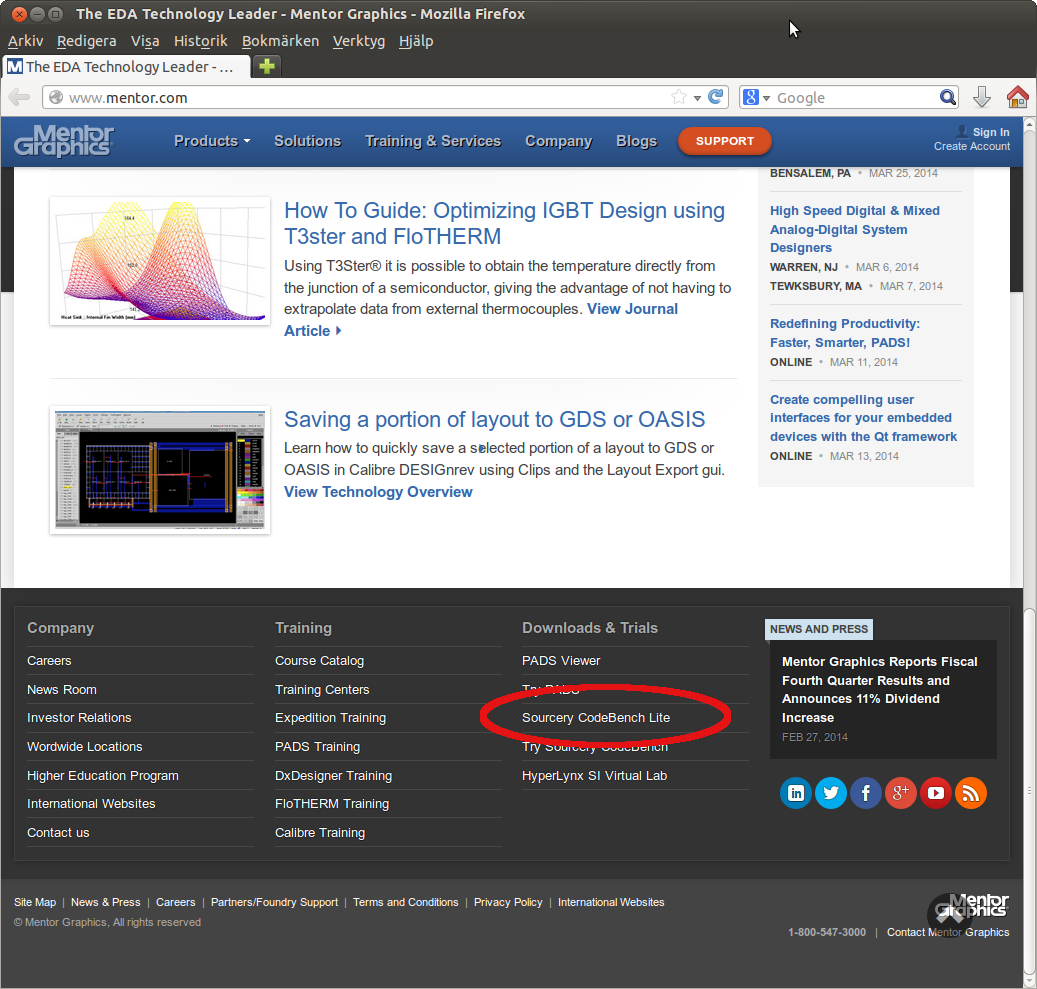
\includegraphics[width=\textwidth]{labs/codesourcery/Mentor_Homepage.png}
\end{center}

Go to the bottom and open the \href{http://www.mentor.com/embedded-software/sourcery-tools/sourcery-codebench/editions/lite-edition.html}{Sourcery Codebench Lite} page
\clearpage

Once on the page, select the \href{http://www.mentor.com/embedded-software/sourcery-tools/sourcery-codebench/editions/lite-edition/arm-gnu-linux.html}{Download the Gnu/Linux Release} for the ARM processor.
\\

\begin{center}
  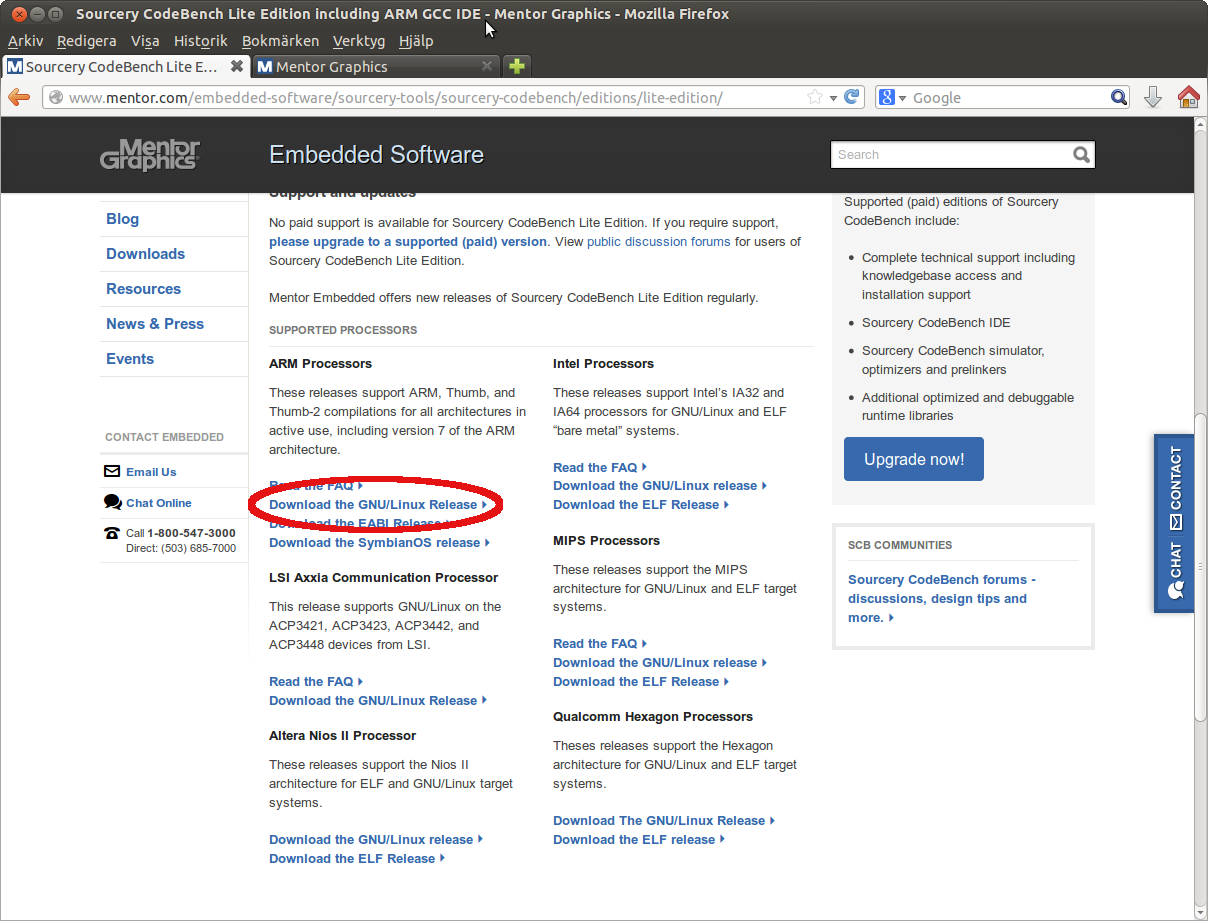
\includegraphics[width=\textwidth]{labs/codesourcery/Gnu_Linux.png}
\end{center}
\clearpage

Fill in your personal details and click the {\bf Get Lite!} button.
\\

\begin{center}
  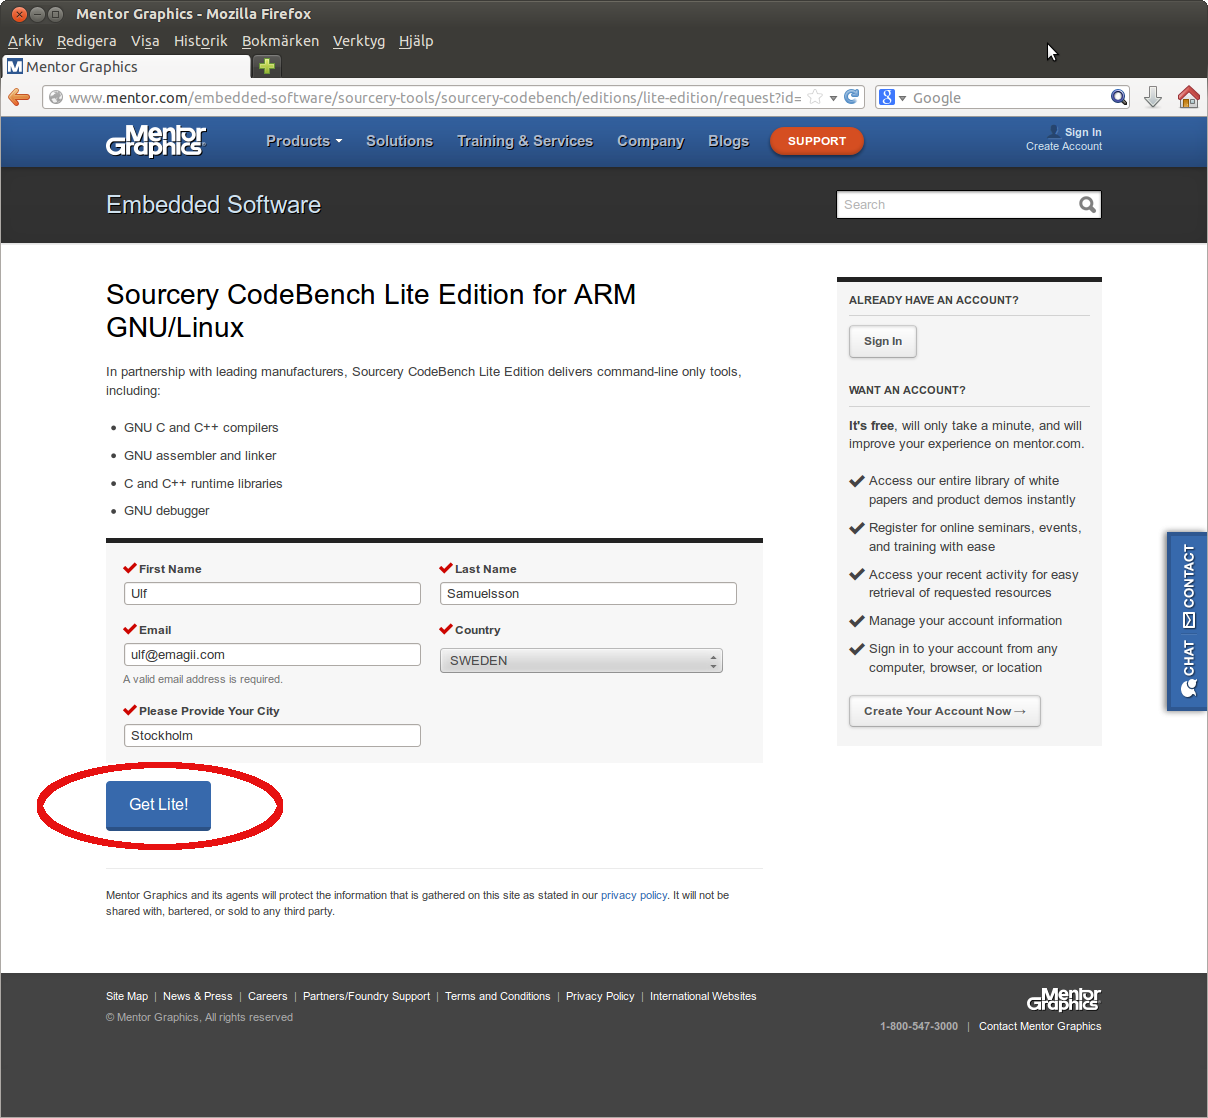
\includegraphics[width=\textwidth]{labs/codesourcery/Mentor_User_Info.png}
\end{center}

You will get a mail with the download location.
Click on the link in the mail and you will open a page from where
you can select your download.
\clearpage

Select the \codesourcery version


\begin{center}
  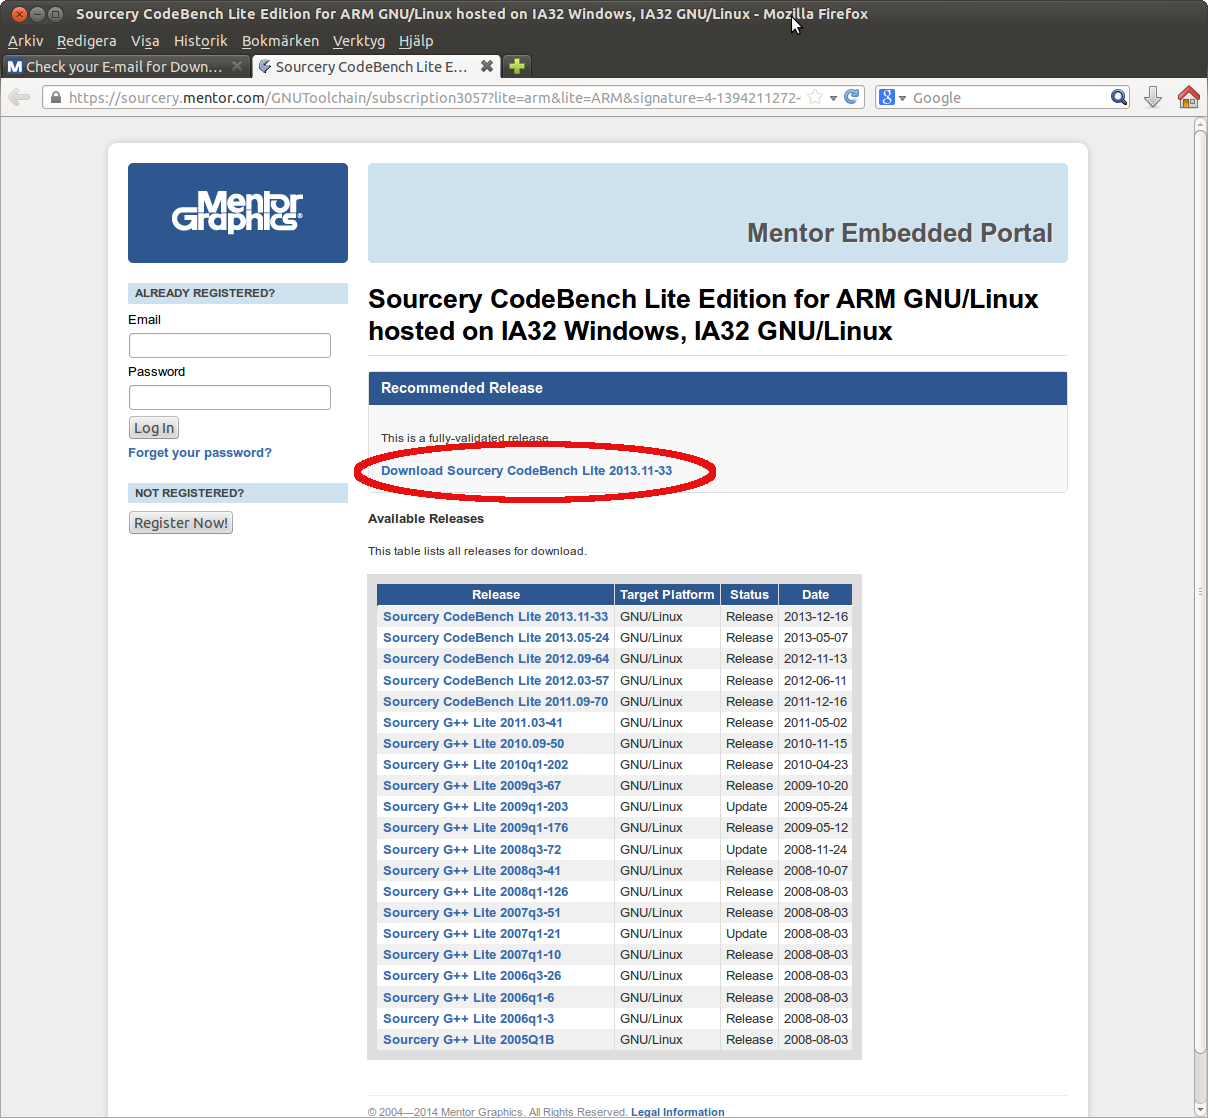
\includegraphics[width=\textwidth]{labs/codesourcery/Codebench_Lite_2013_11.png}
\end{center}
\clearpage

Right Click the {\bf IA32 GNU/Linux Installer} and save at an appropriate place.

\begin{center}
  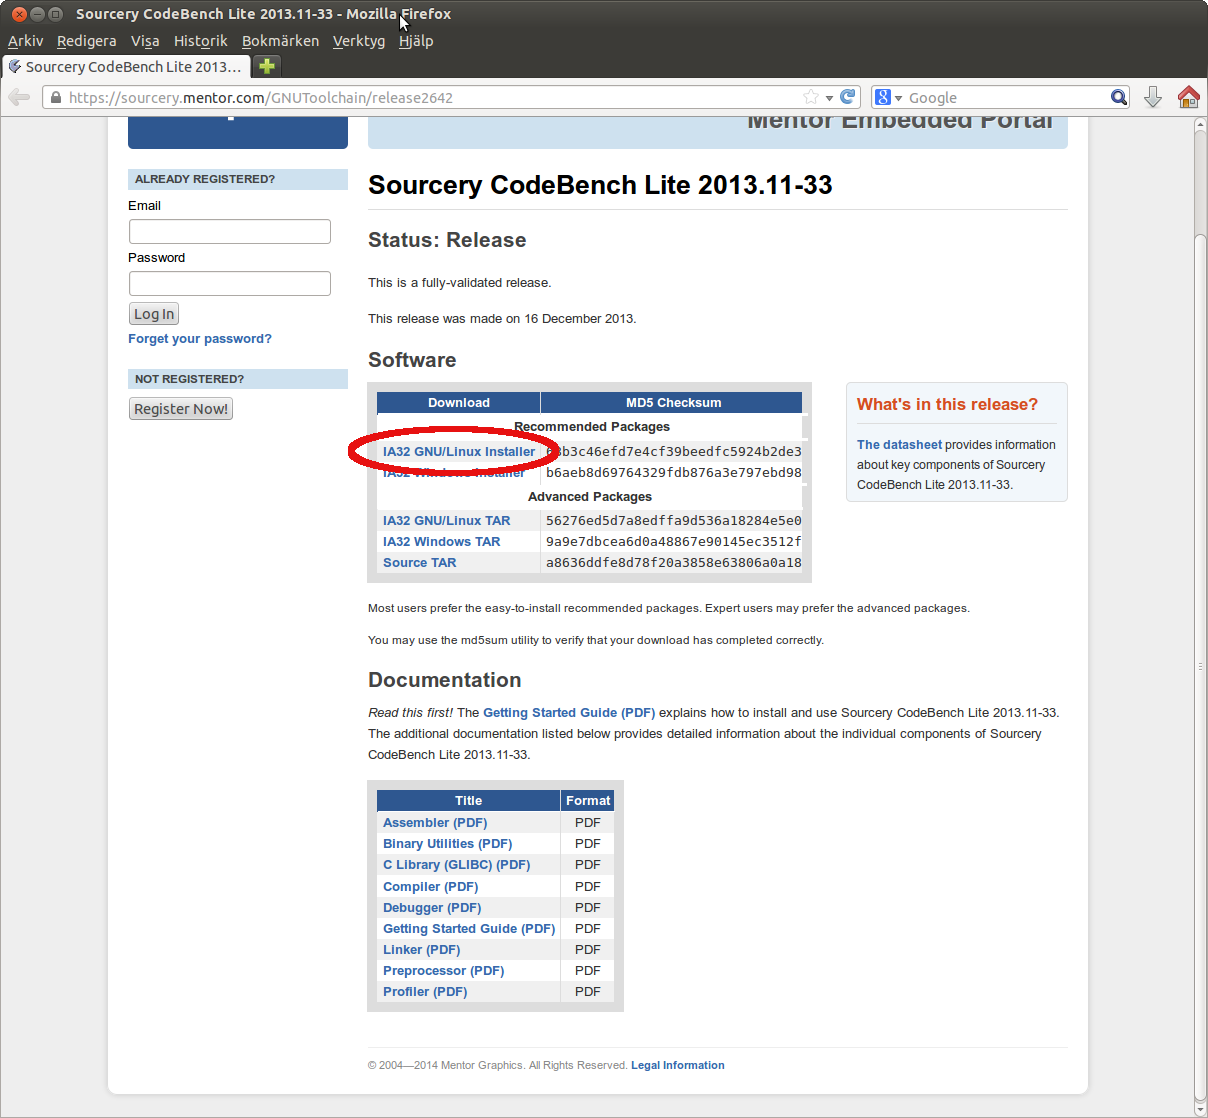
\includegraphics[width=\textwidth]{labs/codesourcery/Codebench_Lite_2013_11_Gnu-Linux.png}
\end{center}

{\bf Getting-Started.pdf} contains the installation guide and should also be downloads.

You may also want to download the rest of the documentation.

\clearpage
\section{Installing the Sourcery Codebench Lite}

Go to the directory where you downloaded the Installer and make it executable.

\code{chmod a+x arm-2013.11-33-arm-none-linux-gnueabi.bin}

Run the installer

\code{./arm-2013.11-33-arm-none-linux-gnueabi.bin}

The installer should be pretty obvious. If not, use the {\bf Getting-Started.pdf} guide.

After the Installation, the path must be set up.

Edit \code{"~/.bashrc"} and add the path to the Installation.

\code{export PATH=<install-dir>/bin:$PATH}

You may also want to create a file \code{sourcery.sh} to source for setting up the toolchain.
\begin{verbatim}
#!/bin/sh
export ARCH=arm
export GCCROOT=<install-dir>
export PATH=$GCCROOT/bin:$PATH
export CROSS_COMPILE=arm-none-linux-gnueabi-
\end{verbatim}

Make sure it is executable:

\code{chmod a+x sourcery.sh}

And then source it.

\code{. ./sourcery.sh}

Check the setup by checking the version of the C-Compiler.

\code{arm-none-linux-gnueabi-gcc --version}

Your output should be similar to:

\begin{verbatim}
arm-none-linux-gnueabi-gcc (Sourcery CodeBench Lite 2013.11-33) 4.8.1
Copyright (C) 2013 Free Software Foundation, Inc.
This is free software; see the source for copying conditions.  There is NO
warranty; not even for MERCHANTABILITY or FITNESS FOR A PARTICULAR PURPOSE.

\end{verbatim}

Verify that the first line of the output contains: Sourcery CodeBench Lite 2013.11-33.

Whenever you need to run the Sourcery CodeBench Lite toolchain, you should source
the \code{sourcery.sh} file to set up the environment.






